\documentclass[dvipdfmx,12pt]{beamer}
%\documentclass[dvipdfmx,12pt,handout]{beamer}
\usepackage{pxjahyper}
\usepackage{minijs}
\usepackage{otf}
\renewcommand{\kanjifamilydefault}{\gtdefault}
\useoutertheme{infolines}
\usecolortheme[RGB={0,128,0}]{structure}
\usecolortheme{dolphin}
\setbeamertemplate{navigation symbols}{}
\setbeamercolor{frametitle}{fg=white, bg=gray}

\title{ダブルオークション設計}
\author{小川慶将}
\date{\today}

\begin{document}
\begin{frame}\frametitle{}
 \titlepage
\end{frame}

\begin{frame}\frametitle{発表の流れ}
 \tableofcontents
\end{frame}

\section{シングルオークションとは}
\subsection{夏合宿の復習}
\begin{frame}
\frametitle{シングルオークションとは}
\begin{itemize}\setlength{\parskip}{0.5em}
\item
売り手1人に対して、買い手が複数人存在。(逆も然り)\\
Yahooのオークションとかがこのタイプ。
\item
主に4種に分類される。
\begin{itemize}\setlength{\parskip}{0.5em}
\item
イングリッシュ・オークション(価格上昇オークション)
\item
ダッチ・オークション(価格下落オークション)
\item
ファーストプライス封印オークション
\item
セカンドプライス封印オークション
\end{itemize}
\end{itemize}
\end{frame}

\section{ダブルオークションとは}
\subsection{ダブルオークション概要}
\begin{frame}
\frametitle{ダブルオークションとは}
\begin{columns}[t]
\begin{column}{0.6\textwidth} % 左:60%
\begin{itemize}\setlength{\parskip}{0.5em}
\item<1->
売り手複数人に対して、買い手も複数人存在。\\
均衡価格は需要曲線と供給曲線の交点となる。
\item<2->
日本では「ザラバ」と呼ばれることもある。\\
株式市場とかで使われいる。
\item<3->
このような需給の均衡はどのように達成されるのだろうか。\\
また、需要曲線や供給曲線って何者なんだろうか。
\end{itemize}
\end{column}
\begin{column}{0.4\textwidth}
\begin{figure}
\centering
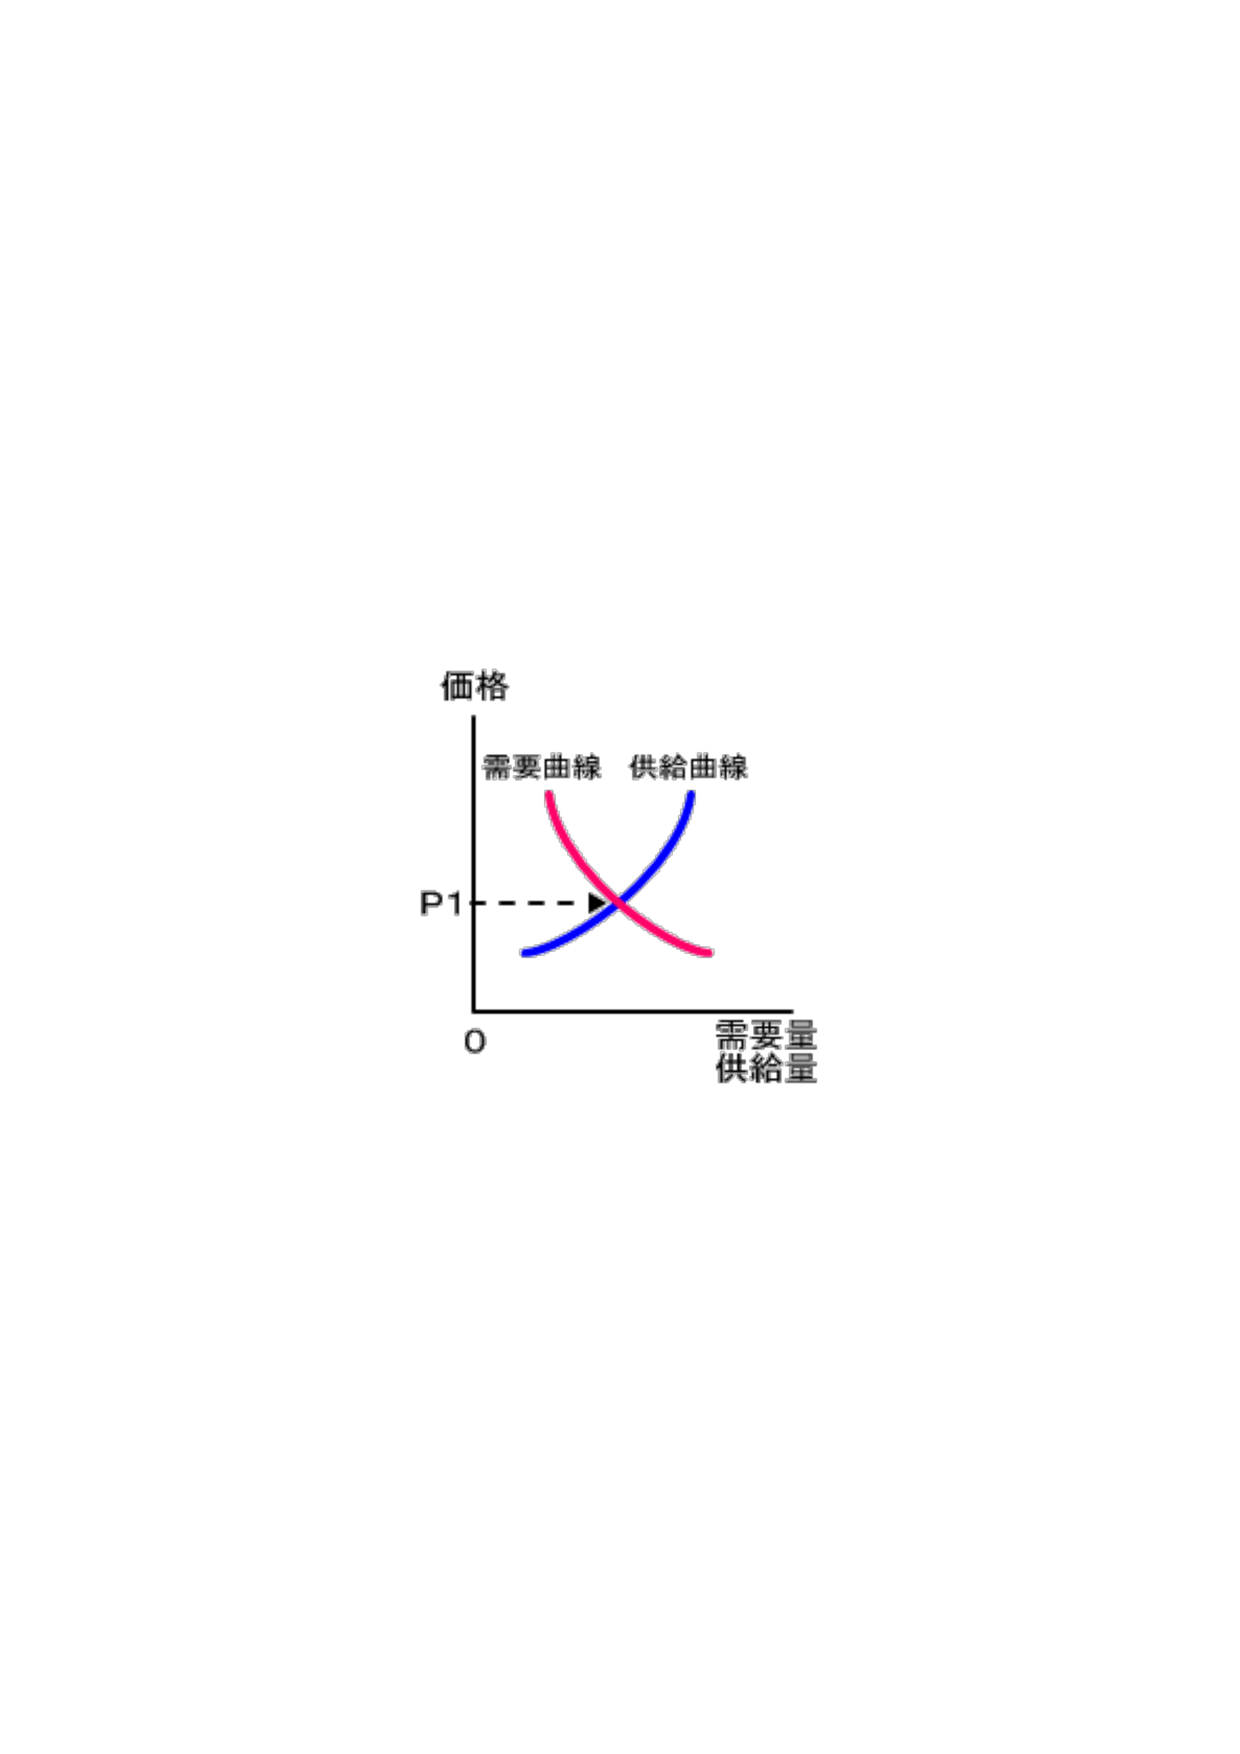
\includegraphics[width=50mm]{juyou-kyoukyu.pdf}
\caption{需要曲線と供給曲線}
\label{fig:jukyuu}
\end{figure}
\end{column}
\end{columns}
\end{frame}

\begin{frame}
\frametitle{供給曲線・需要曲線の導出}
\begin{itemize}\setlength{\parskip}{0.5em}
\item
例えば以下のような私的情報を持つ売り手6人、買い手6人がいたとする。

売り手:13 18 19 20 21 30\\
買い手:30 24 23 22 18 14
\end{itemize}
\end{frame}

\begin{frame}
\frametitle{供給曲線の導出}
\begin{itemize}\setlength{\parskip}{0.5em}
\item
売り手:13 18 19 20 21 30
\end{itemize}
\begin{figure}
\centering
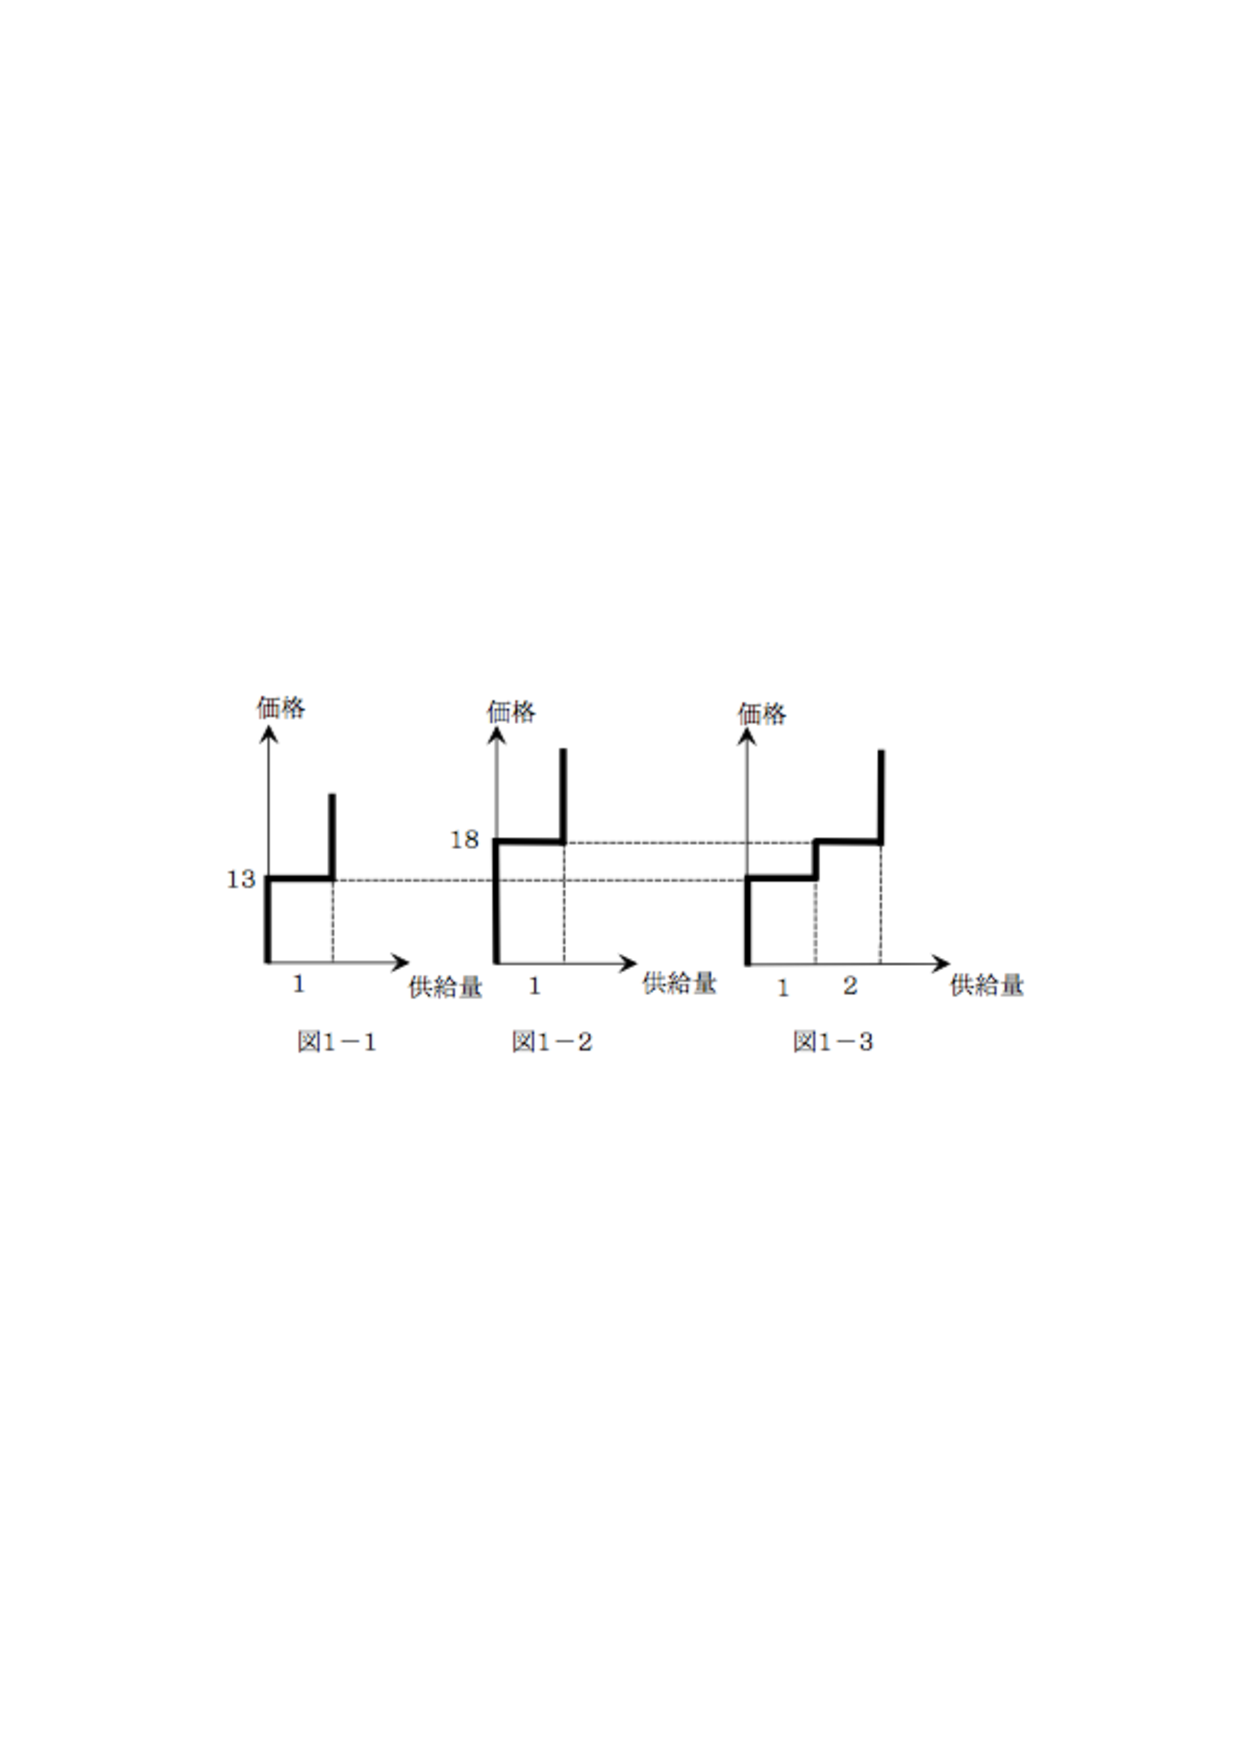
\includegraphics[width=100mm]{supply.pdf}
\caption{供給曲線の導出}
\label{fig:supply}
\end{figure}
\end{frame}

\begin{frame}
\frametitle{需要曲線の導出}
\begin{itemize}\setlength{\parskip}{0.5em}
\item
買い手:30 24 23 22 18 14
\end{itemize}
\begin{figure}
\centering
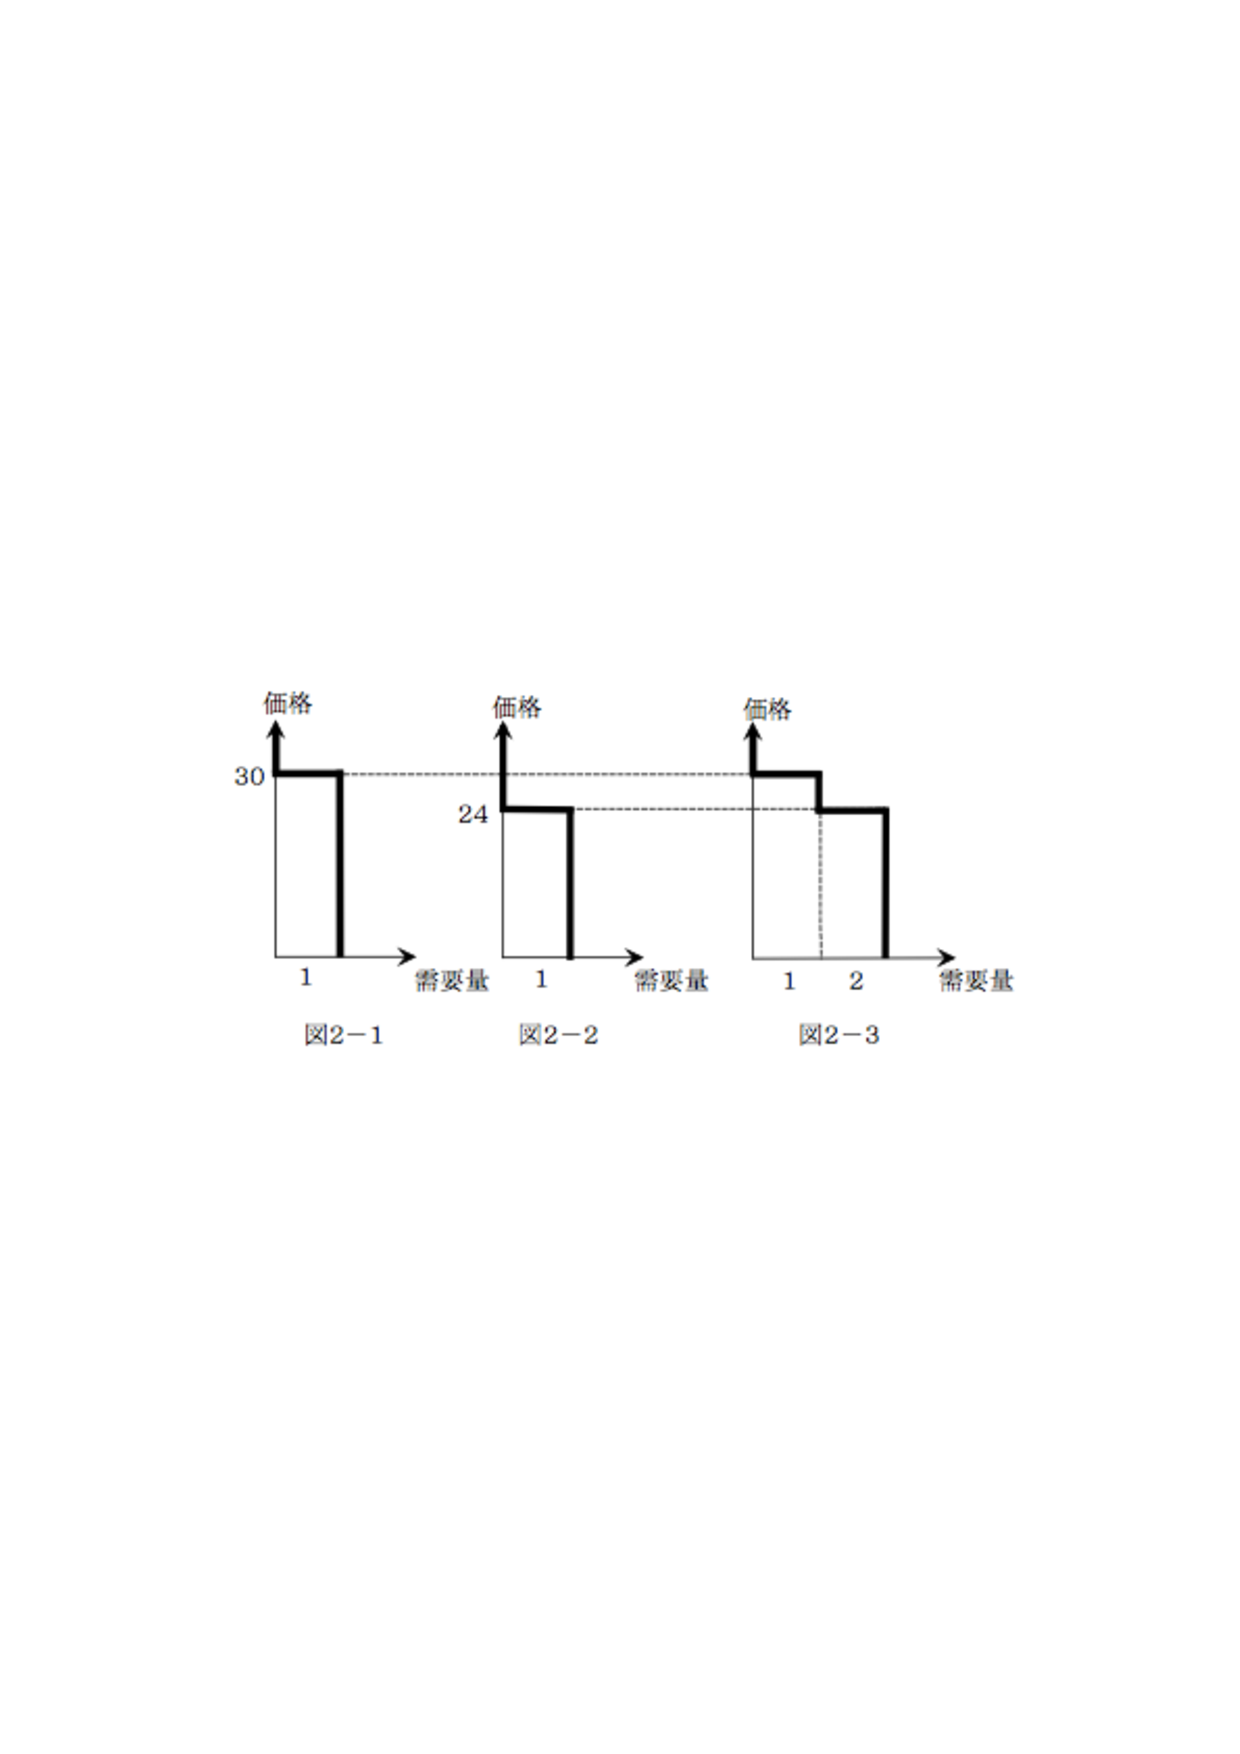
\includegraphics[width=100mm]{demand.pdf}
\caption{需要曲線の導出}
\label{fig:demand}
\end{figure}
\end{frame}

\begin{frame}
\frametitle{供給曲線と需要曲線}
\begin{itemize}\setlength{\parskip}{0.5em}
\item
売り手:13 18 19 20 21 30\\
買い手:30 24 23 22 18 14
\item
均衡価格は 20 〜 21 円 の間のどこか。\\
均衡取引量は4単位。\\
総余剰は30+24+23+22-13-18-19-20 = 29円。
\end{itemize}
\begin{figure}
\centering
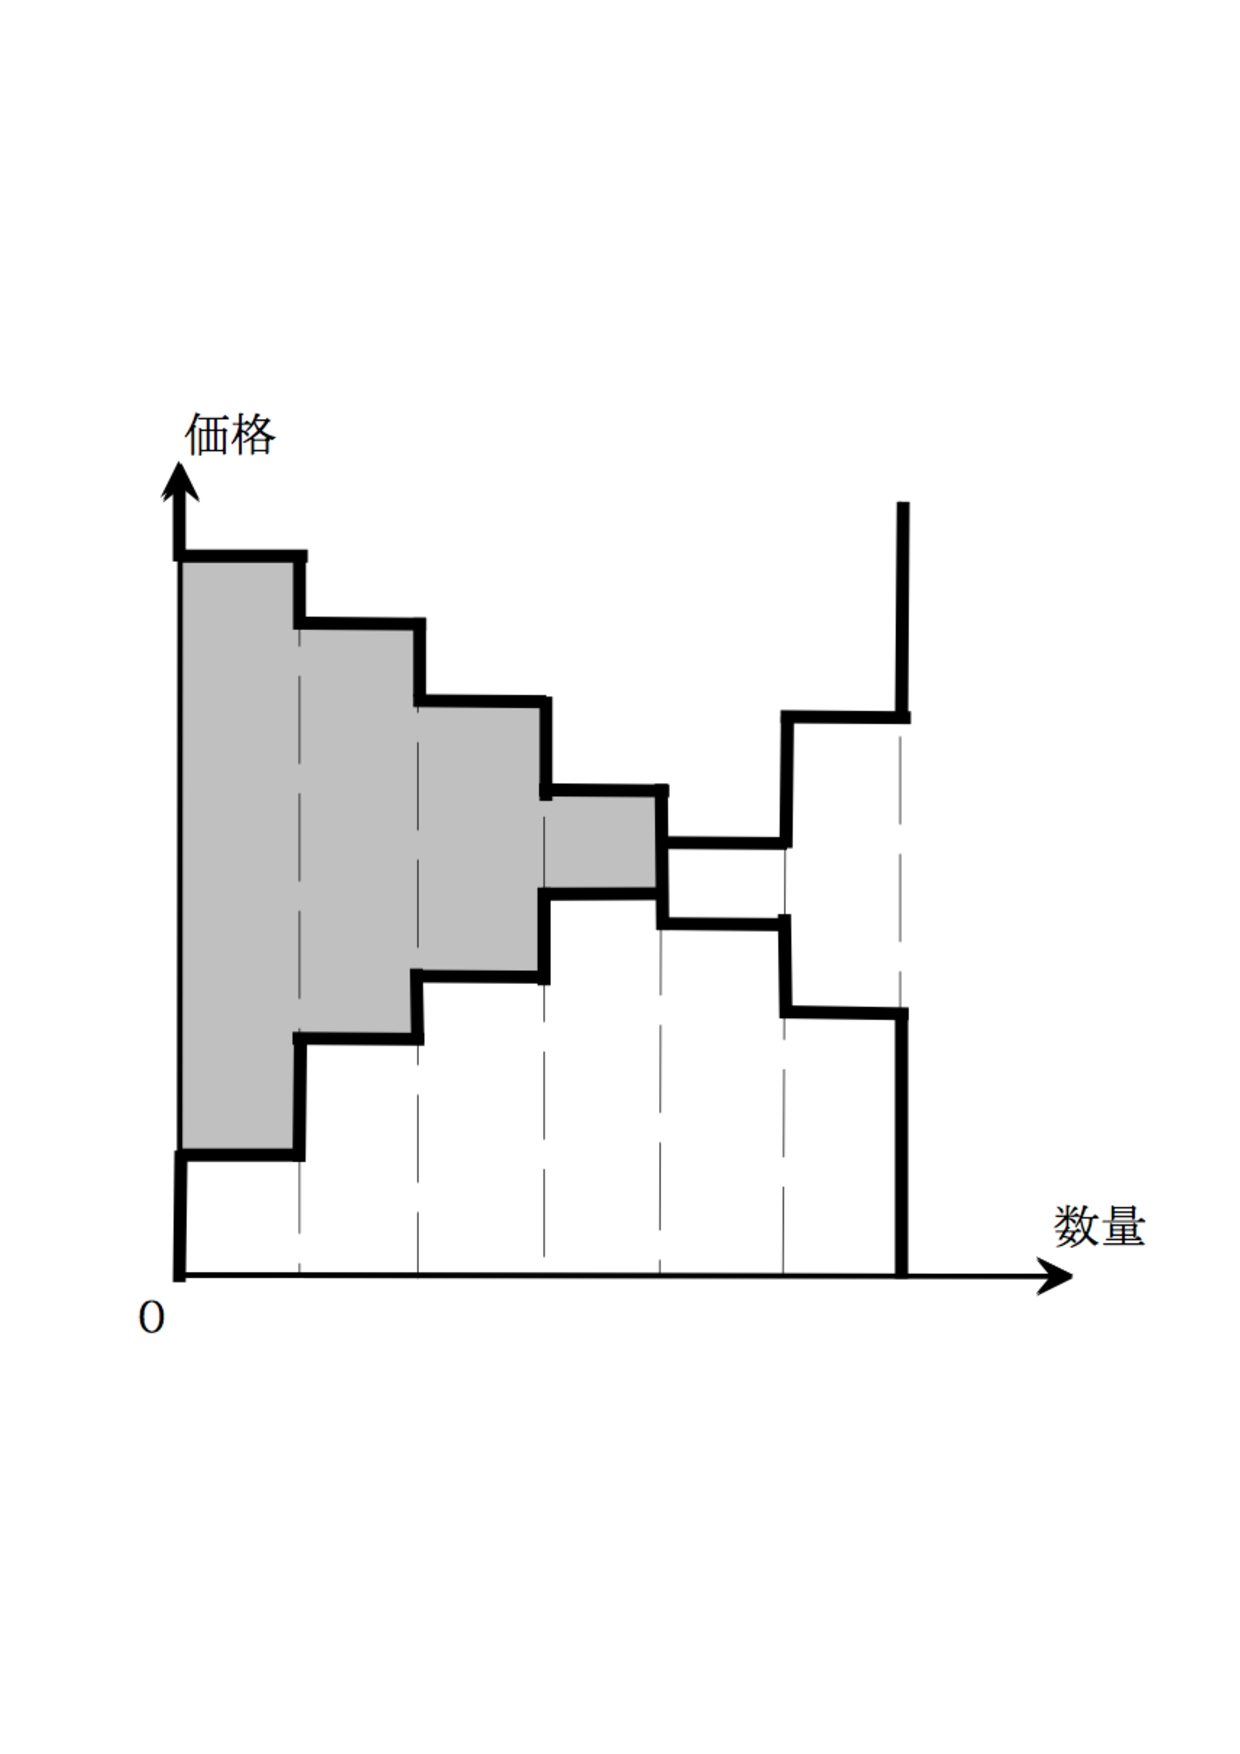
\includegraphics[width=40mm]{price.pdf}
\caption{供給曲線と需要曲線}
\label{fig:price}
\end{figure}
\end{frame}

\subsection{チェンバリン実験}
\begin{frame}
\frametitle{チェンバリン実験デザイン(ピットマーケット)}
\begin{itemize}\setlength{\parskip}{0.5em}
\item
私的情報を生徒12人(売り手6人、買い手6人)に与えて、\\
よーいドン!で教室内でお互いの取引を許す。\pause
\item
生徒が知る情報は自分の私的情報のみで、\\
この市場における需要曲線、供給曲線などは知らない。\pause
\item
5分後に取引タイム終了の合図を出して結果報告。
\end{itemize}
\end{frame}

\begin{frame}
\frametitle{チェンバリン実験結果(ピットマーケット)}
\begin{itemize}\setlength{\parskip}{0.5em}
\item
実験結果はいかに...\pause
\item
取引量が均衡取引量を上回る結果に。\\
理由:買い手も売り手も自分の私的情報しか知らないので、取引できそうな人に出会うと即成約させようとしてしまうからであろう。\pause
\item
取引量が均衡取引量を上回るということは、\\
総余剰も均衡時より小さく経済効率を損ねている状態である。\pause
\item
チェンバリンはこの実験結果をもとに、\\
完全競争下における市場の理論が機能しないものとした。
\end{itemize}
\end{frame}

\subsection{スミス実験}
\begin{frame}
\frametitle{スミス実験デザイン(ダブルオークション)}
\begin{itemize}\setlength{\parskip}{0.5em}
\item
チェンバリンの実験デザインは、個々の取引での情報が非効率的にしか共有されていないのではないか。\pause
\item
じゃあ、全ての買値、売値を公開しながら取引を行えばどうなるんだろうか。\pause
\item
買い手、売り手は手を挙げ実験者からの指名を受けた後、\\
価格情報を全員に対して公開する。\pause
\item
例えば、売り手が指名を受け、24円で売りたいと言ったとする。\pause
\item
それに対して、\\
24円より安く売っても良いと思っている売り手、\\
24円なら買いたいと思っている買い手が手を挙げる。\pause
\item
これを繰り返して取引を成立させていく。
\end{itemize}
\end{frame}

\begin{frame}
\frametitle{スミス実験結果(ダブルオークション)}
\begin{itemize}\setlength{\parskip}{0.5em}
\item
実験結果はいかに...\pause
\item
ほぼ均衡時と同じ取引量、価格になる。\pause
\item
ここにおいて、需給の法則が成立する価格の決定方法と取引の手続きという具体的な制度を発見した。\pause
\item
ここでは参加者は他の参加者の私的情報を全て知っている訳ではない。\\
にも関わらず、容易に均衡へ達することが出来る。\pause
\item
教科書に書いてあるような「完全情報」の定義は強すぎることも分かった。\\
\end{itemize}
\end{frame}

\begin{frame}
\frametitle{コラム:完全競争市場って何人から?}
\begin{itemize}\setlength{\parskip}{0.5em}
\item
完全競争市場で需給の法則が成立するためには、大勢の買い手と売り手が存在しないといけないと教科書には書かれている。\pause
\item
では、いったい何人くらいは最低限必要なの?\pause
\item
買い手、売り手が各々4,5人いれば実は成立することをスミスが発見!\\
何万人もの買い手や売り手が必要になるわけではない。
\end{itemize}
\end{frame}


\section{Pythonコード}
\subsection{willow復習}
\begin{frame}
\frametitle{willowの使い方}
\begin{itemize}\setlength{\parskip}{0.5em}
\item
同じディレクトリにwillowフォルダ、logフォルダを用意する。
\item
from willow.willow import *をコード内に記述。
\end{itemize}
\end{frame}

\subsection{willow復習}
\begin{frame}
\frametitle{主な関数}
\begin{itemize}\setlength{\parskip}{0.5em}
\item
add()\\
主にhtmlを開く際に使う。
\item
take(), put()\\
クライアント同士の情報を受け渡す際に使う。
\item
show(), hide()\\
画面の情報を更新するために使う。
\end{itemize}
\end{frame}

\subsection{実験開始}
\begin{frame}
\frametitle{実験について}
\begin{itemize}\setlength{\parskip}{0.5em}
\item
スミスの実験デザインであるダブルオークションを再現する。
\item
実際にやってみる。
\end{itemize}
\end{frame}

\subsection{コード説明}
\begin{frame}
\frametitle{コード説明}
\begin{itemize}\setlength{\parskip}{0.5em}
\item
別画面にてコードを解説。
\end{itemize}
\end{frame}

\section{まとめ}
\subsection{今後の課題}
\begin{frame}
\frametitle{雑感と課題}
\begin{itemize}\setlength{\parskip}{0.5em}
\item
willowを通じてのhtmlとpythonとの連携に限界が見え始める・・・\\
需要曲線と供給曲線のグラフをブラウザに表示させるなどしたい。\pause
\item
エージェントをプログラム内部に組み込む。\\
エージェントに人工知能を搭載させる。\\
→重たくなるのでより綺麗なコードを書くか言語を検討
\end{itemize}
\end{frame}


\subsection{次回発表案(仮)}
\begin{frame}
\frametitle{次回発表案(仮)}
\begin{itemize}\setlength{\parskip}{0.5em}
\item
「人工市場の創造」\\
\pause
(参考:和泉潔著『人工市場』(2003年、相互作用科学シリーズ)\pause
\item
そのためには、遺伝的アルゴリズムを組み込んだエージェント作成や優れたGUIの実装が必要となる。\pause
\item
とりあえずpythonとwillowを使って限界まで挑戦してみる。
\end{itemize}
\end{frame}

\subsection{参考文献}
\begin{frame}
\frametitle{参考文献}
\begin{itemize}\setlength{\parskip}{0.5em}
\item
『バーノンスミス教授の業績』(西條辰義,2002年)\\
http://www.iser.osaka-u.ac.jp/~saijo/pdffiles/smith.pdf
\item
『実験経済学の事始め』(松島斉,2007年)
http://www.econexp.org/hitoshi/07kotohajime.pdf
\item
『実験経済学入門』(濱口泰代,2010年)
http://www.econ.nagoya-cu.ac.jp/~yhamagu/20100930jikken1.pdf
\end{itemize}
\end{frame}




\end{document}